\begin{pastexam}[label={px:ccu-110-csb-04}]{中正資工所乙組 110 學年度 第 4 題}
（問答）

(25\%) Consider the following undirected graph. Please answer the following questions.
\begin{enumerate}[label=(\alph*)]
\item (5\%) Please write down the sequences of edges selected by Kruskal's algorithm.
\item (5\%) Please write down the sequences of edges selected by Prim's algorithm (start from
vertex A).
\item (15\%) Let $G$ denote a given undirected graph with positive edge weights such as the
following graph. Please prove that if each edge in $G$ has a \textbf{distinct} weight, then there
will be only one \textbf{unique} minimum cost spanning tree in $G$ by contradiction.
\end{enumerate}

\begin{center}
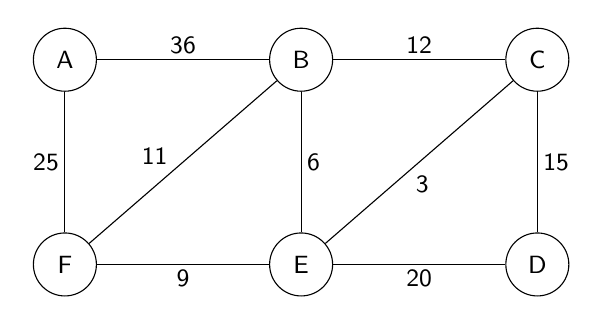
\begin{tikzpicture}[v/.style={circle,draw,minimum size=8mm,inner sep=0pt,font=\sffamily\small},w/.style={font=\sffamily\small,inner sep=2pt}]
\node[v] (A) at (0,2.6) {A};
\node[v] (B) at (3,2.6) {B};
\node[v] (C) at (6,2.6) {C};
\node[v] (F) at (0,0) {F};
\node[v] (E) at (3,0) {E};
\node[v] (D) at (6,0) {D};
\draw (A) -- node[w,above] {36} (B);
\draw (B) -- node[w,above] {12} (C);
\draw (A) -- node[w,left] {25} (F);
\draw (B) -- node[w,above left,pos=0.55] {11} (F);
\draw (B) -- node[w,right] {6} (E);
\draw (C) -- node[w,below right,pos=0.55] {3} (E);
\draw (C) -- node[w,right] {15} (D);
\draw (F) -- node[w,below] {9} (E);
\draw (E) -- node[w,below] {20} (D);
\end{tikzpicture}
\end{center}
\end{pastexam}

\begin{pastsoln}
\textbf{(a)} 九條邊依權重由小到大：C--E（$3$）、B--E（$6$）、E--F（$9$）、B--F（$11$）、
B--C（$12$）、C--D（$15$）、D--E（$20$）、A--F（$25$）、A--B（$36$）。

\begin{center}
\small
\begin{tabular}{rcrll}
\toprule
步 & 邊 & 權重 & 結果 & 處理完的集合 \\
\midrule
1 & C--E & 3 & 選 & $\{C, E\}$ \\
2 & B--E & 6 & 選 & $\{B, C, E\}$ \\
3 & E--F & 9 & 選 & $\{B, C, E, F\}$ \\
4 & B--F & 11 & 略過：B、F 已經經過 E 連通 & $\{B, C, E, F\}$ \\
5 & B--C & 12 & 略過：B、C 已經經過 E 連通 & $\{B, C, E, F\}$ \\
6 & C--D & 15 & 選 & $\{B, C, D, E, F\}$ \\
7 & D--E & 20 & 略過：D、E 已經經過 C 連通 & $\{B, C, D, E, F\}$ \\
8 & A--F & 25 & 選，已滿 $5$ 條 & $\{A, B, C, D, E, F\}$ \\
\bottomrule
\end{tabular}
\end{center}

Kruskal 選邊的順序是 (C, E)、(B, E)、(E, F)、(C, D)、(A, F)，總權重
$3 + 6 + 9 + 15 + 25 = 58$。

\textbf{(b)} 從 A 開始執行 Prim 演算法，每回合取出 $\mathit{key}$ 最小的頂點（格子寫
$\mathit{key}/\pi$，空白表示已在樹裡）：

\begin{center}
\small
\begin{tabular}{cccrrrrrr}
\toprule
回合 & 取出 & 加入的邊 & A & B & C & D & E & F \\
\midrule
1 & A & — & $0$ & $36/A$ & $\infty$ & $\infty$ & $\infty$ & $25/A$ \\
2 & F & A--F & & $11/F$ & $\infty$ & $\infty$ & $9/F$ & $25/A$ \\
3 & E & F--E & & $6/E$ & $3/E$ & $20/E$ & $9/F$ & \\
4 & C & E--C & & $6/E$ & $3/E$ & $15/C$ & & \\
5 & B & E--B & & $6/E$ & & $15/C$ & & \\
6 & D & C--D & & & & $15/C$ & & \\
\bottomrule
\end{tabular}
\end{center}

（每一列是取出那個頂點、更新完鄰居之後的值；取出的頂點那一格是它被取出時的值。） 第 4 回合
C 的 B--C 是 $12$，不比 $\mathit{key}[B] = 6$ 小，不更新。 Prim 選邊的順序是 (A, F)、(F, E)、
(E, C)、(E, B)、(C, D)，和 (a) 是同一組邊，總權重 $58$；九條邊權重都不同，最小生成樹唯一。

\textbf{(c)} 證明（反證法）。 設 $G$ 是連通的無向圖，$n$ 個頂點，每條邊的權重都不同。 假設 $G$
有兩棵不同的最小生成樹 $T_1 \ne T_2$。

\begin{enumerate}
\item 兩棵都是生成樹，都恰好有 $n - 1$ 條邊（資結書定理~21.3）。 邊數一樣而集合不同，
所以 $T_1$ 有不在 $T_2$ 裡的邊，$T_2$ 也有不在 $T_1$ 裡的邊。 令
$D = (T_1 - T_2) \cup (T_2 - T_1)$，是「恰好屬於其中一棵」的邊，$D \ne \emptyset$。
\item 權重互不相同，$D$ 裡權重最小的邊 $e$ 是唯一的。 不失一般性，設 $e \in T_1$、$e \notin T_2$
（否則把 $T_1$、$T_2$ 的名字對調）。
\item 把 $e = (u, v)$ 加進 $T_2$。 $T_2$ 裡 $u$ 到 $v$ 本來就有一條簡單路徑 $P$，加上 $e$ 形成
一個環 $C = P \cup \{e\}$。
\item $P$ 上一定有一條邊 $f$ 不在 $T_1$ 裡。 否則 $P$ 的邊全在 $T_1$ 裡，連同 $e \in T_1$，
環 $C$ 整個在 $T_1$ 裡，和 $T_1$ 是樹（沒有環）矛盾。
\item $f \in T_2$、$f \notin T_1$，所以 $f \in D$；$f$ 在 $P$ 上而 $e$ 不在 $T_2$ 裡，所以
$f \ne e$。 由 $e$ 是 $D$ 裡唯一最輕的邊，$w(f) > w(e)$。
\item 令 $T' = T_2 - \{f\} \cup \{e\}$。 從 $T_2$ 拿掉 $f$，樹分成兩塊；$f$ 在 $u$ 到 $v$ 的路徑
$P$ 上，所以 $u$、$v$ 分在不同的兩塊，加上 $e$ 又連成一棵樹。 $T'$ 是生成樹，而且
\[
w(T') = w(T_2) - w(f) + w(e) < w(T_2),
\]
和 $T_2$ 是最小生成樹矛盾。
\end{enumerate}
所以假設不成立，權重互不相同時最小生成樹只有一棵。 這就是資結書定理~24.4。 注意題
目說的「positive edge weights」在證明裡沒有用到，權重是負數也成立。

\end{pastsoln}
